
\documentclass[../D+Manual.tex]{subfiles}
\begin{document}

\chapter{Examples} \label{chp:examples}

\begin{quote}
	Few things are harder to put up with than the annoyance of a good example.\\
	\hspace*{\fill} \textit{Mark Twain}
\end{quote}

D+ is very dynamic. Demonstrating all the options combinations would be near impossible. Examples of how to use scripts can be found in the \path{./LuaScripts/} directory. Other examples, which were discussed in the paper and its SOM can be found in the \path{./Example Files/} directory, where D+ is installed. The folder contains 7 subfolders. Each folder, contains a \texttt{*.state} file that can be loaded to D+. After the \texttt{state} file is loaded, pressing \texttt{Generate} will compute the scattering curve.  The expected result is also provided as an \texttt{*.out} file. Here, we shall present two examples of models: one real and PDB based; and one for fun and to demonstrate the great flexibility of D+.

\section{Microtubles}

The original reason D+ was developed was to model microtubules at resolutions that matched the SAXS data.
Microtubles are comprised of $\alpha\beta$ tubulin heterodimers arranged as a tube on a helical lattice.
There are many PDBs of the tubulin dimer.
We shall use a modified PDB file of the tubulin dimer located in the \path{./Example Files/4_Microtubule} directory: \path{3j6f_Dimer_2_2_Added_H_GCentered.pdb}.
The PDB file is aligned such that the long axis is roughly parallel to the $z$ axis (details about the alignment of atomic structures can be found in the supporting online materials (SOM) of  \cite{Dplus2017}).

Load the PDB (in the \hyperref[sec:domainView]{\texttt{Domain View}}).
The PDB is already centered, so checking or unchecking the Center PDB checkbox will have no effect.
To make the multiple copies of tubulin that are needed to construct a microtubule, add the \path{Super Helical Left Hand MT Helix.lua} scripted symmetry located in the \path{./LuaScripts/} directory. In the \hyperref[sec:domainView]{\texttt{Domain View}}, drag the PDB line onto the \texttt{Super Helical Left Hand MT Helix} line. This tells D+ to use the script to make multiple copies of the tubulin dimer.

To better understand how the \hyperref [sec:ScriptedSymmetry]{\texttt{Scripted Symmetry}} works, play around with the parameters. Then look at the code.
You can see the code of a loaded 
\hyperref [sec:ScriptedSymmetry]{\texttt{Scripted Symmetry}} in the \hyperref [sec:symmetryEditor] {\texttt{Script Editor}} by double clicking on the script name in the \hyperref[sec:domainView]{\texttt{Domain View}}.

Now, let us correct the model. Select the \texttt{Super Helical Left Hand MT Helix} in the \hyperref[sec:domainView]{\texttt{Domain View}}. Enter the parameters from the table in the \hyperref[sec:parameterEditor]{\texttt{Parameter Editor}}. These are roughly the correct parameters for microtubules. Pressing \texttt{Generate} (in the \hyperref[sec:controls]{\text{Controls}} pane) may or may not give an accurate scattering pattern (depending on parameters like \texttt{Grid Size}, \texttt{Convergence}, and \texttt{Integration Iterations}), as the object is long and artifacts will occur (see Chapter \ref{chp:reciprocalGrids} for details).
 
\begin{wraptable}{r}{0.45\textwidth}
	\vspace{-20pt}
	\centering
	\begin{tabularx}{0.95\linewidth}{X l}
		\toprule
		\textbf{Parameter} & \textbf{Value}\\
		\midrule
		Radius & 11.94 \\
		Pitch & 12.195 \\
		Units per Pitch & 14 \\
		Units in Pitch & 14 \\
		Discrete Height & 36 \\
		\# Helix Starts & 3 \\
		Super Helical Pitch & 0 \\
		\bottomrule
	\end{tabularx}
\end{wraptable}

\section{Interim Results}\label{sec:IntRes}
Assume that in the previous section, you did not choose to integrate using VEGAS nor opted to use the \hyperref[sec:UsingHybridMethod]{Hybrid Method}.
These choices are important for reasons that will be explained below.
There are two results besides the actual scattering curves once the generate button has been pressed.
First, as we constructed a larger atomic model from a PDB file and a symmetry, one might want a PDB file of the entire structure.
This PDB file can be obtained by selecting the symmetry whose PDB file you want and then under the \texttt{File} menu choosing \texttt{Export PDB Representation}.
The PDB file is constructed using the parameters when the generate button is pressed, so if you change the parameters after pressing generate, the resulting file may not be what you would expect.

The second result that can save computation time later, is the scattering amplitude of any of the elements in the tree (in this case either the PDB model or the \hyperref [sec:ScriptedSymmetry]{\texttt{Scripted Symmetry}}). Amplitude can be saved under the \path{File} menu, by pressing on \path{Export Amplitude File...}. If the tree has more than one model, pressing on each model before exporting the amplitude, will save the amplitude of the chosen model. If models are under \texttt{Manual Symmetry}, pressing on the \texttt{Manual Symmetry} or on any of the models in it, before exporting the amplitude, will save the amplitude grid of the entire symmetry. 



A saved amplitude (RG) can be loaded as an \texttt{Amplitude Grid (AMP)} in the \hyperref[sec:domainView]{\texttt{Domain View}} pane.
This \texttt{Amplitude Grid} saves the computation time of that (sub)structure in the future as the interim result can be loaded and inserted in other structures as well.

When using the \hyperref[sec:VEGAS]{\texttt{Adaptive (VEGAS) Monte Carlo}} integration method, all the calculations are carried out on the GPU without transferring the interim results back to the CPU.
Once the computation is complete, the interim results are lost. In particular, the \texttt{Amplitude Grid} file (an \texttt{AMP} file) cannot be exported. 
Similarly, when using the \hyperref[sec:UsingHybridMethod]{\texttt{Hybrid Method}}, no RG is created for nodes whose \texttt{Use Grid From Here} checkbox is unchecked and therefore it cannot be saved.

\section{Stick Figure}
Make a stick figure. For the head, add a sphere, for the body, a cylinder, etc. Use this picture as a guide. Try to use both geometric shapes and symmetries (manual and space-filling). The method we used can be found in \path{./Example Files/D+Man.state}.
There is no scientific value to this structure, it is just a way to practice manipulating objects in D+.

\begin{wrapfigure}{r}{0.2\textwidth}
	\vspace{-20pt}
	\centering
	%l b r t
	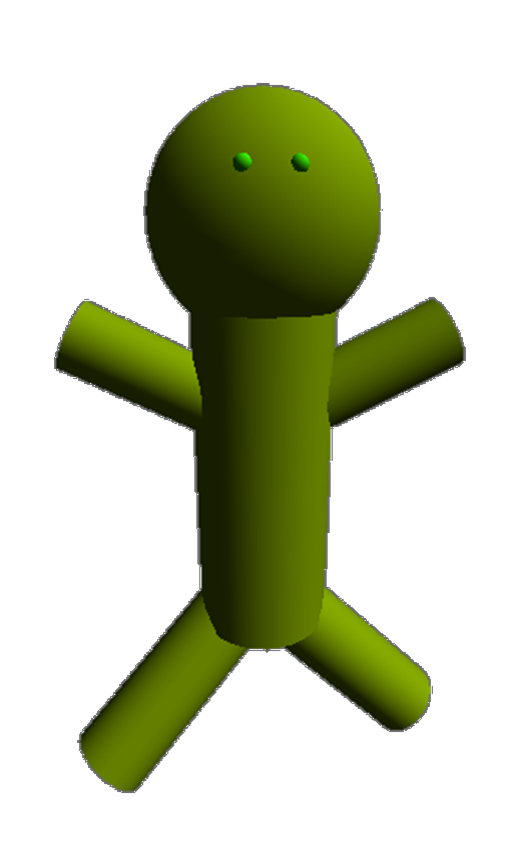
\includegraphics[width=0.95\linewidth]{D+WhiteMan2}
\end{wrapfigure}

\end{document}